\sloppy
\documentclass[14pt,a4paper,oneside]{extarticle}	% Размер основного шрифта и формата листа
\usepackage{xltxtra}						% Используется для вывода логотипа XeLaTeX
\usepackage{xunicode}						% Кодировка документа
\usepackage{polyglossia}					% Загружает пакет многоязыковой верстки
\newfontfamily\russianfont{Book Antiqua}
%\setmainfont{Liberation Serif}						% Основной шрифт текста
\setmainfont{Book Antiqua}
\setdefaultlanguage{russian}				% Основной язык текста
\setotherlanguage{english}					% Дополнительный язык текста
\linespread{1}							% Межстрочный интервал выбран полуторным
\usepackage[left=2.5cm,
right=1.5cm,vmargin=2.5cm]{geometry} % Отступы по краям листа
\bibliographystyle{ugost2008}

\usepackage{xcolor}
\usepackage{hyperref}
% Цвета для гиперссылок
\definecolor{linkcolor}{HTML}{359B08} % цвет ссылок
\definecolor{urlcolor}{HTML}{799B03} % цвет гиперссылок
\hypersetup{pdfstartview=FitH,  linkcolor=linkcolor,urlcolor=urlcolor, colorlinks=true}

%---------------------------%
%---- Пакеты расширений ----%
%---------------------------%
\usepackage{xcolor}
\usepackage{hyperref}
% Цвета для гиперссылок
\definecolor{linkcolor}{HTML}{359B08} % цвет ссылок
\definecolor{urlcolor}{HTML}{799B03} % цвет гиперссылок
\hypersetup{pdfstartview=FitH,  linkcolor=linkcolor,urlcolor=urlcolor, colorlinks=true}


\usepackage{verbatim,indentfirst}
\usepackage{cite,enumerate,float}
\usepackage{amsmath,amssymb,amsthm,amsfonts}

%---------------------------%
%--- Вставка иллюстраций ---%
%---------------------------%
\usepackage{graphicx}
\usepackage{subfigure}
%\graphicspath{{Images/}}
\usepackage{fontspec}

\begin{document}
%	\pagestyle{empty} %  выключаенм нумерацию
%\setcounter{page}{3}% Нумерация начинается с третьей страницы
%\renewcommand{\contentsname}{\center{Содержание}}
%\tableofcontents

\begin{center}
%	\addcontentsline{toc}{section}{Опыт 18.«Прыгающий шарик»}
	\subsection*{Переход потенциальной энергии в кинетическую и обратный переход}
\end{center}

\begin{figure}[H] 
	\centering 	
	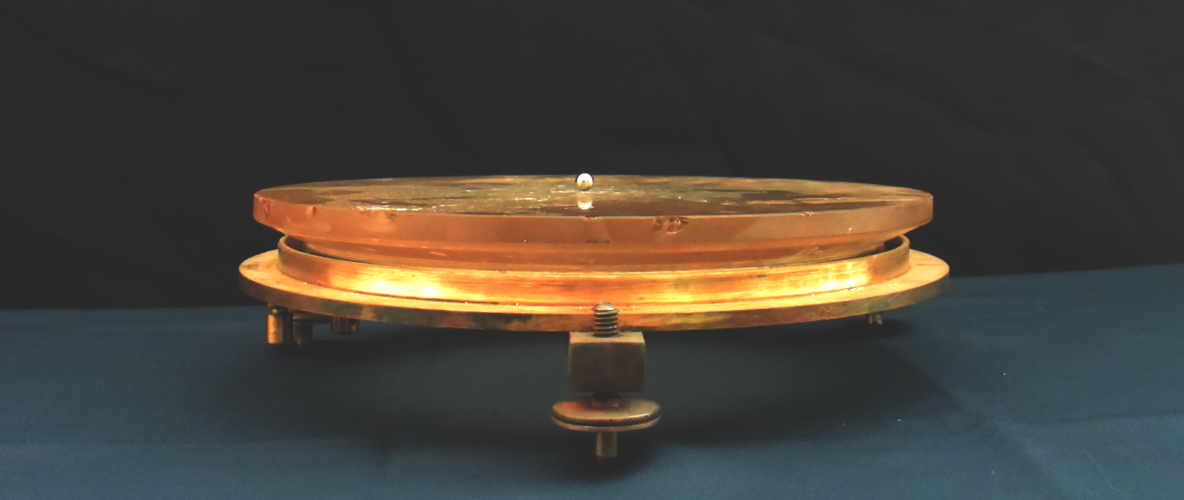
\includegraphics[width=0.8\linewidth]{transform-1.png}
	\caption{Демонстрация превращения потенциальной энергии в кинетическую на примере «прыгающего» шарика}
	\label{transform-1}
\end{figure}

\subsection*{\underline{Оборудование:}}

\begin{enumerate}
	\item Стеклянная линза диаметром 25 см 
	\item Стальной шарик диаметром 5-6 мм
	\item Подставка с юстировочными винтами
\end{enumerate}

\subsection*{\underline{Основные определения:}}

Сумма потенциальной и кинетической энергий системы тел 
получила название полной энергии системы: 
$$
	W=E_\text{к} + E_\text{п}
$$

Полная энергия системы определяет ту работу, которую можно 
получить от данной системы тел при ее взаимодействии о какими-либо другими телами, не входящими в эту систему. 

При движении тел изолированной системы только 
под действием внутренних сил полная энергия системы не изменяется. 
При таких движениях тел происходит только превращение части 
потенциальной энергии в кинетическую.
В этом и состоит закон 
сохранения энергии, который можно сформулировать следующим 
образом:  
\textit{\begin{flushleft}
	в изолированной системе тел полная энергия остается постоянной во все время движения тел; в системе происходят лишь превращения энергии из одного вида в другой. 
\end{flushleft}}

\subsection*{\underline{Краткое описание:}}

В рамках этой демонстрации можно наблюдать переход потенциальной энергии в кинетическую и обратно с потерей некоторой части энергии вследствие не вполне упругого удара.
Перед демонстрацией опыта опора, на которой
плоской поверхностью кверху помещена линза, при помощи юстировочных винтов выставляется в горизонтальное положение.
Тогда стальной шарик, отпущенный без начальной скорости с некоторой высоты над линзой, отскочит строго вертикально вверх, а не в разные стороны.
В таких условиях шарик будет прыгать до тех пор, пока не растратит весь запас механической энергии.
Опыт также можно проводить в теневой проекции или бросив шарик вдоль открытой с двух концов стеклянной трубки.

\begin{figure}[H] 
	\centering 	
	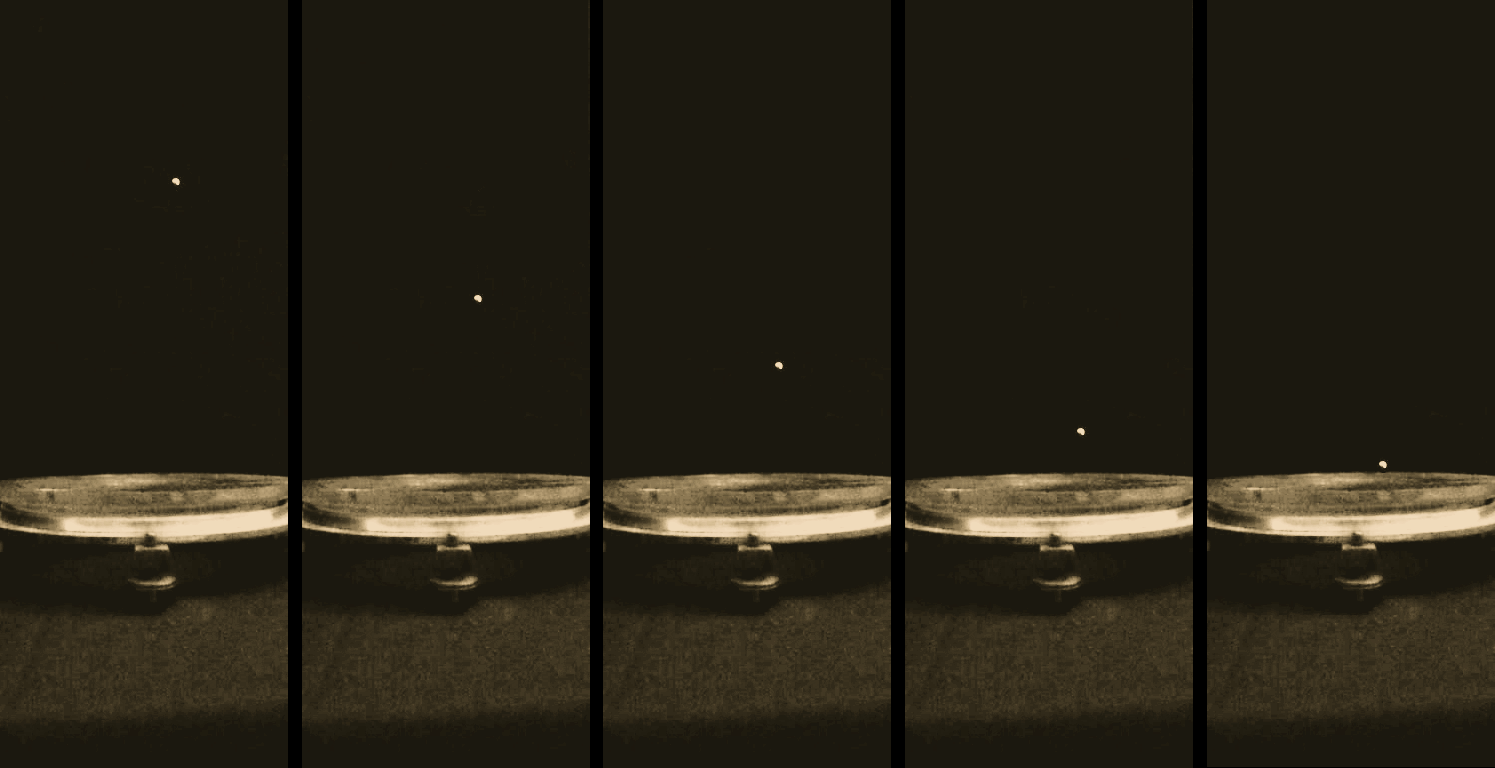
\includegraphics[width=0.9\linewidth]{transform-2.png}
	\caption{Демонстрация потери механической энергии прыгающего на стеклянной линзе стального шарика}
	\label{transform-2}
\end{figure}

\newpage

\subsection*{\underline{Теория:}}

Рассмотрим вначале, что происходить с энергией изолированной системы, если телам предоставить возможность свободно двигаться под действием внутренних сил. 

Пусть тело массы \textit{m} находится на высоте $ h_1 $ над поверхностью 
Земли и не имеет начальной скорости (рис.\ref{transform-3}). 
В этом положении тело будет обладать потенциальной энергией $ E_\text{п}=mgh_1 $, но не будет иметь кинетическую энергию, $ E_\text{к}=0 $. 
%$ E_\text{к}=mv_1^2 $

Полная механическая энергия численно будет равна потенциальной $W = E_\text{п} =mgh_1$.

\begin{figure}[H] 
	\centering 	
	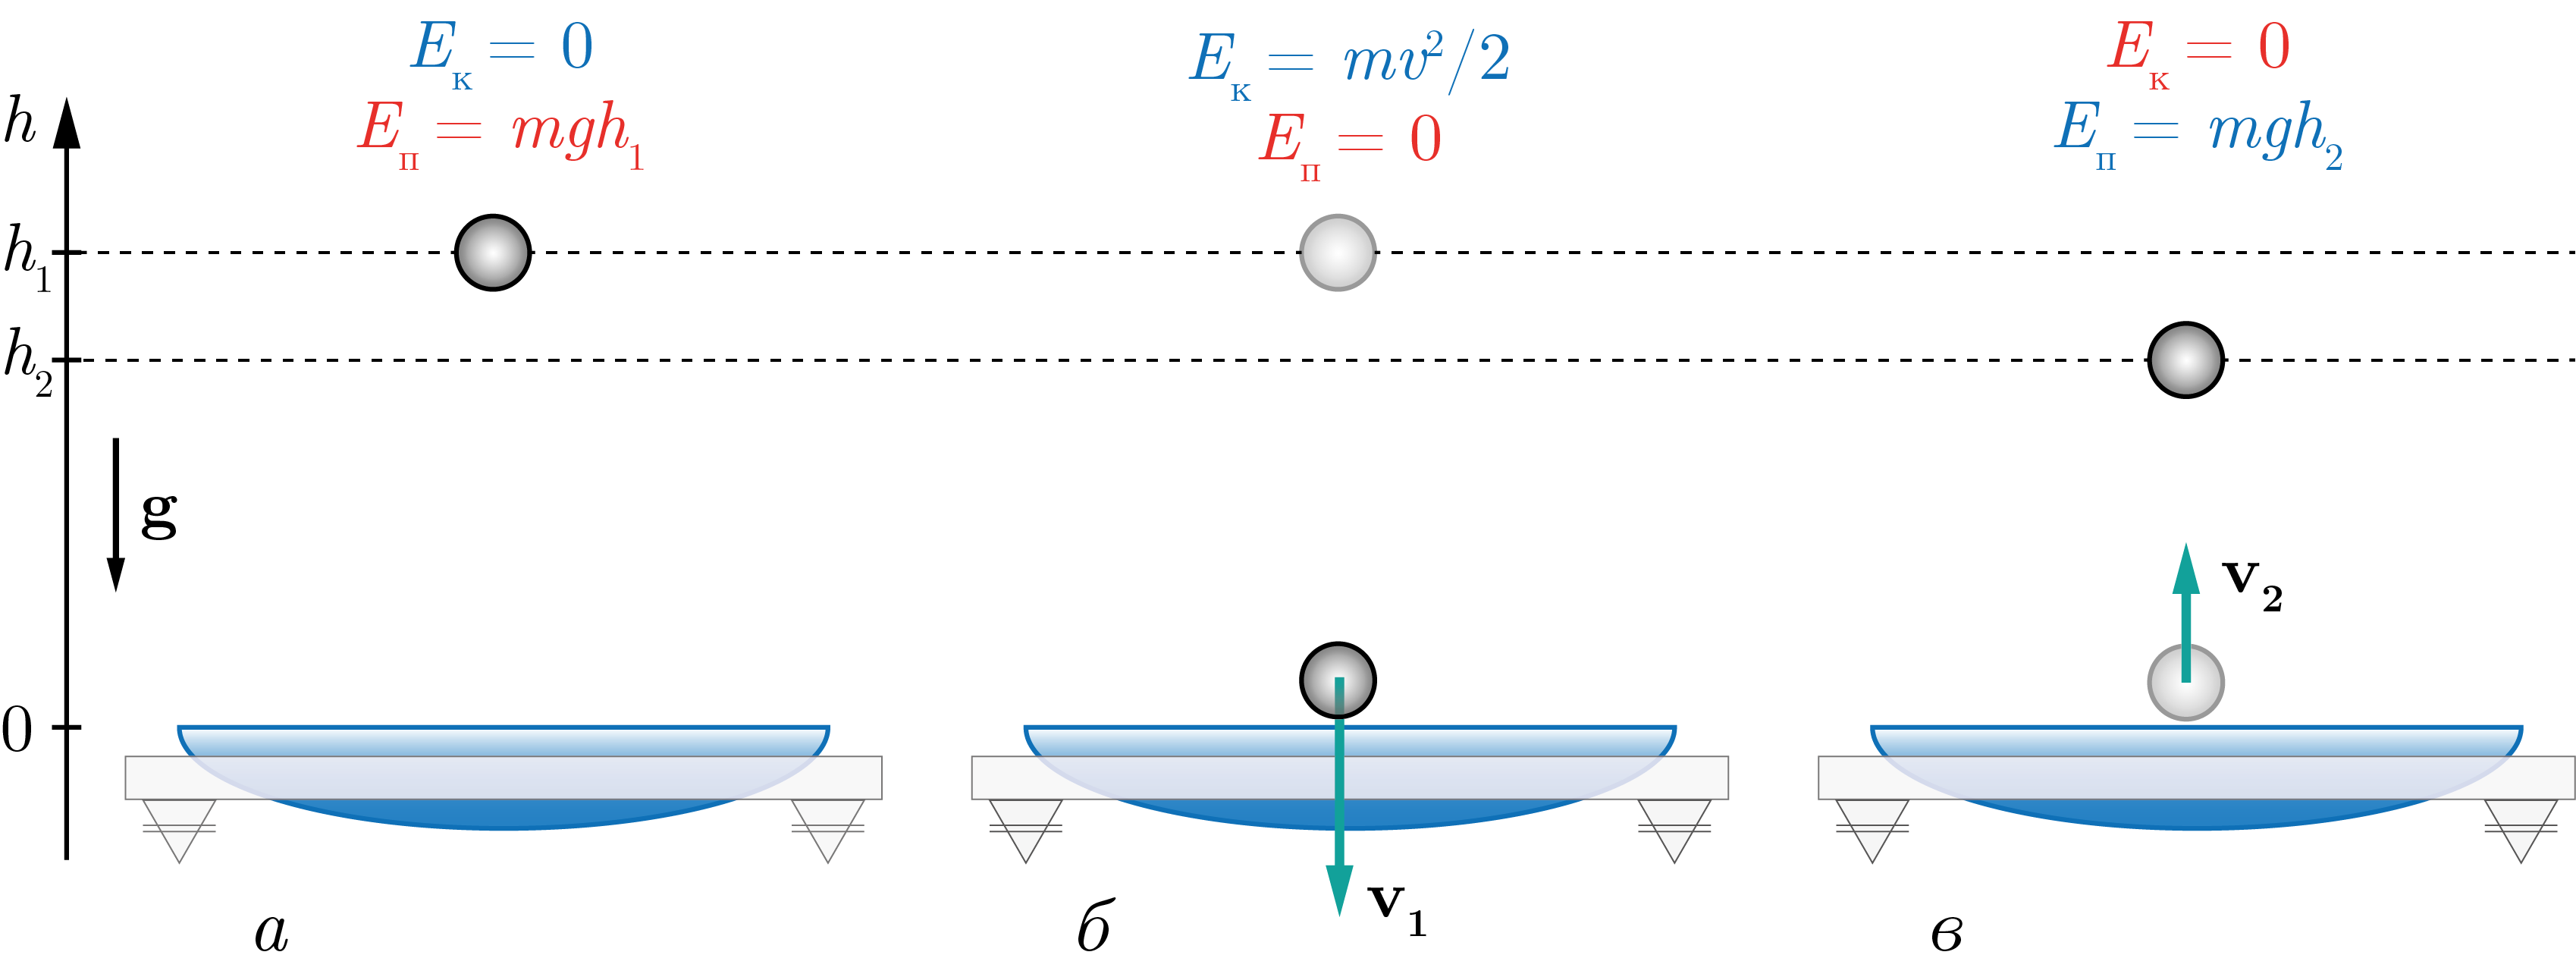
\includegraphics[width=0.9\linewidth]{transform-3.png}
	\caption{Демонстрация превращения потенциальной энергии в кинетическую и обратного превращения}
	\label{transform-3}
\end{figure}

Допустим, что тело опустилось на некоторую высоту и его скорость увеличилась (в самой нижней точке скорость тела возрастет до $ v_1 $).
При таком движении сила тяжести совершит работу
\begin{equation}
\Delta A=mgh_1.
\end{equation}

Вся эта работа $ \Delta A  $ будет израсходована на увеличение кинетической энергии тела: 
\begin{equation}
\Delta A=mv_1^2.
\end{equation}
при условии, что трения и внешних сил не было. 

Подставляя в это выражение значение работы $ \Delta A $, можно получить: 
\begin{equation}
mgh_1=mv_1^2.
\end{equation}

Левая часть полученного выражения определяет полную энергию системы для начального момента времени (в рассматриваемом случае тело обладает только потенциальной энергией), 
а правая — полную энергию системы для конечного момента времени, когда тело приблизилось к земле.

Из закона сохранения полной механической энергии следует, что 
если на систему действуют какие-либо внешние силы, то изменения полной энергии системы равны работе этих внешних сил. 
Если в системе действуют силы трения, то полная энергия системы при движении тел уменьшается.
Она расходуется на работу против этих сил.
Одновременно работа сил трения приводит к нагреву системы.
Как известно, при работе сил трения происходит превращение механического движения в тепловое.
Количество выделившегося тепла при этом в точности равно убыли полной механической энергии системы. 

Возвращаясь к опыту с шариком, при падении его начальная потенциальная энергия перейдет в кинетическую 
энергию вблизи поверхности линзы, где потенциальная энергия равна нулю.
После отскока шарик начнет движение вверх, и при подъеме кинетическая энергия тела начнет 
превращаться в потенциальную энергию, зависящую от высоты шарика.
Если трения нет, тело, двигаясь вверх, 
должно подняться до начальной высоты \textit{h}.
Такой процесс падения и последующего подъема должен был бы повторяться неограниченно много раз при условии отсутствия трения. 

Постепенное уменьшение высоты подъема шарика при многократном отскоке от линзы, которое можно 
наблюдать в ходе опыта (рис.\ref{transform-2}), полностью объясняется потерями энергии на 
трение.
Другими словами полная механическая энергия \textit{W} в такой системе не сохраняется.

Для рассматриваемой системы также применимо понятие коэффициента восстановления  при ударе \textit{k}.
Если известны высота $ h_1 $, с которой тело начинает движение без начальной скорости, и высота $ h_2 $ подъема шарика после удара о массивную плиту, то при помощи формул Галилея
\begin{equation}
\begin{cases}
v_1=\sqrt{2gh_1} \\
v_2=\sqrt{2gh_2}
\end{cases}
\end{equation}
можно получить выражение для определения коэффициента \textit{k}:
\begin{equation}
k=\dfrac{v_2}{v_1}=\sqrt{\dfrac{h_2}{h_1}}.
\end{equation}

\end{document}